\documentclass{beamer}  % presen 12pt
\mode<presentation>
\usepackage{hyperref}
%\usepackage{beamerthemesplit}
%

\input{../../Lab/stylefiles/rules/MyPackages}
% Font
\input{../../Lab/stylefiles/rules/MyBold}
\input{../../Lab/stylefiles/rules/MyCal}
\input{../../Lab/stylefiles/rules/MyScr}
\input{../../Lab/stylefiles/rules/MyBB}
\input{../../Lab/stylefiles/rules/MyTilde}
\input{../../Lab/stylefiles/rules/MyBar}
\input{../../Lab/stylefiles/rules/MyHat}
\input{../../Lab/stylefiles/rules/MyRoman}
% Environment
\input{../../Lab/stylefiles/rules/MyOperations}
\input{../../Lab/stylefiles/rules/MyNewEnvironment}
% References
\input{../../Lab/stylefiles/rules/MyJournals}
\bibliographystyle{IEEEtran}
\usepackage{graphicx}
\usepackage{lscape}
\usepackage{beamerthemesplit}
\setbeamertemplate{navigation symbols}{}
\setbeamertemplate{footline}[frame number]
\usetheme{Luebeck}
\renewcommand{\figurename}{図}
\renewcommand{\tablename}{表}
\usepackage{xeCJK}
\setCJKmainfont{MS Gothic}
%

\input{../../Lab/stylefiles/rules/MyPackages}
% Font
\input{../../Lab/stylefiles/rules/MyBold}
\input{../../Lab/stylefiles/rules/MyCal}
\input{../../Lab/stylefiles/rules/MyScr}
\input{../../Lab/stylefiles/rules/MyBB}
\input{../../Lab/stylefiles/rules/MyTilde}
\input{../../Lab/stylefiles/rules/MyBar}
\input{../../Lab/stylefiles/rules/MyHat}
\input{../../Lab/stylefiles/rules/MyRoman}
% Environment
\input{../../Lab/stylefiles/rules/MyOperations}
\input{../../Lab/stylefiles/rules/MyNewEnvironment}
% References
\input{../../Lab/stylefiles/rules/MyJournals}
\bibliographystyle{IEEEtran}
\usepackage{graphicx}
\usepackage{lscape}
\usepackage{beamerthemesplit}
\setbeamertemplate{navigation symbols}{}
\setbeamertemplate{footline}[frame number]
\usetheme{Luebeck}
\renewcommand{\figurename}{図}
\renewcommand{\tablename}{表}

\title[ターボ符号器における決定論的インタリーバの設計に関する研究]{ターボ符号器における決定論的インタリーバの設計に関する研究}
\author[Bohulu]{Bohulu Kwame Ackah, 1631133}
\institute[UEC]{情報伝送研究室}
\date[Week 3]{\today}

\begin{document}
\frame{\titlepage}

\addtobeamertemplate{navigation symbols}{}{%
    \usebeamerfont{footline}%
    \usebeamercolor[fg]{footline}%
    \hspace{1em}%
    \insertframenumber/\inserttotalframenumber
}

\begin{frame}

	\frametitle{1. ターボ符号について}
	\begin{figure}
		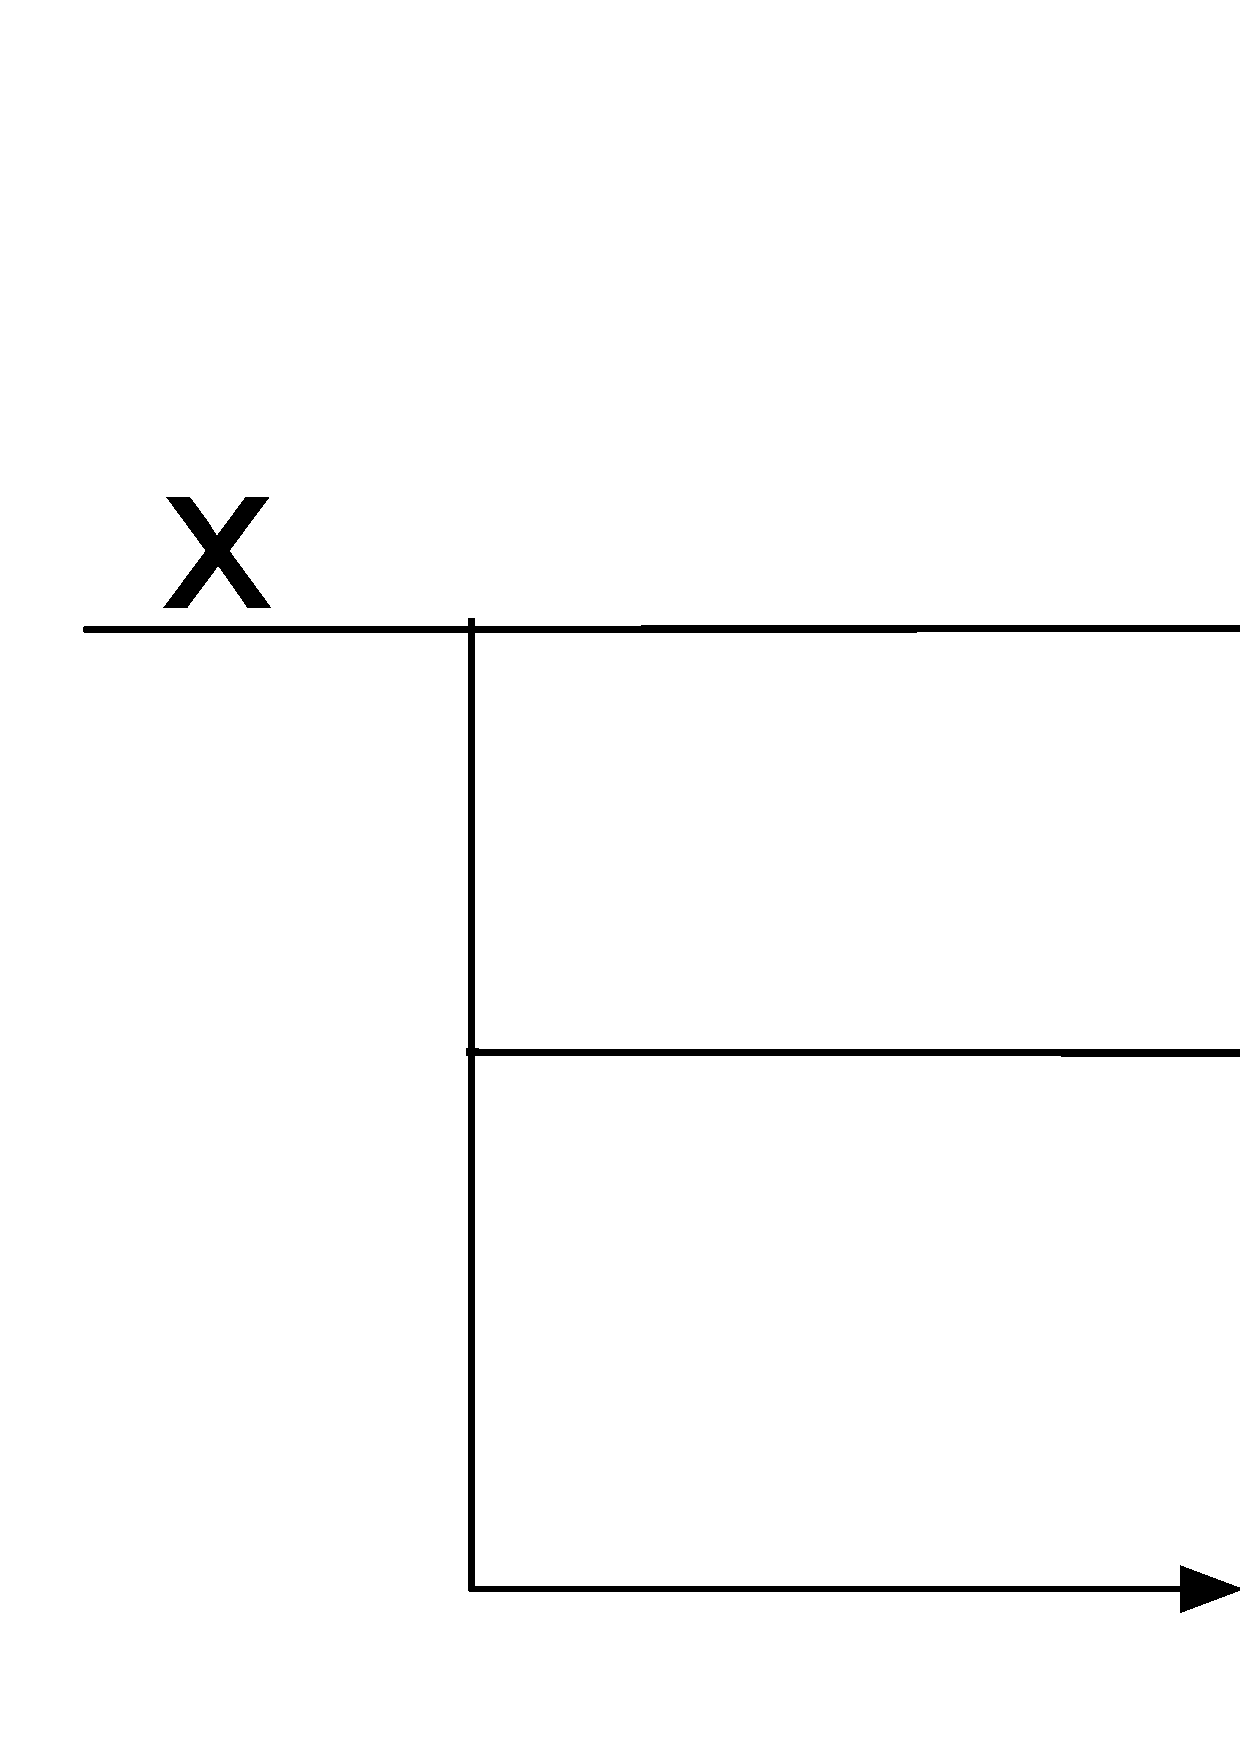
\includegraphics[width=8cm]{TurboEncoder.pdf}
	\end{figure}
	
	\begin{itemize}
	\item AWGNチャネルの通信容量に近い
	\item インタリーバの部分が大変重要
	\end{itemize}
	
\end{frame}

%slide 2

\begin{frame}
\frametitle{2. インタリーバについて}

\begin{itemize}
\setlength\itemsep{2em}
\item 働き:情報系列を並び替えること

\item 二つのグループにわかれている
\begin{itemize}
\setlength\itemsep{1em}
\item ランダムインタリーバ
\begin{itemize}
\item 利点: 長いフレームサイズの場合、性能が良い

\item 欠点: インタリーバテーブルを使用する
\end{itemize}
\item 決定論的インタリーバ
\begin{itemize}
\item 利点: アルゴリズムでインタリーブとデインタリーブができる

\item 欠点:長いフレームサイズの場合、ランダムインタリーバの性能が良い
\end{itemize}
\end{itemize}

\end{itemize}

\end{frame}


\begin{frame}
\frametitle{3. 研究の目的}
\begin{itemize}
\setlength\itemsep{2em}
\item Jing Sun, Oscar Y. Takeshita ”Interleavers for Turbo Codes Using Permutation Polynomials over Integer Rings”, IEEE Trans. Inform. Theory, vol. 51,
pp. 101 - 119 Jan. 2005

\item 本研究の目標: ランダムインタリーバより優れた決定論的インターリーバの開発
%本研究では、長いフレームサイズでランダムインタリーバより優れた決定論的インターリーバの開発を目標としている

%アルゴリズムにより設計できる決定論的インタリーバが、実用に多く採用されている。LTEでは、文献[3]で紹介されているPPIが採用されている。
\end{itemize}
\end{frame}


%slide 3
\begin{frame}
\frametitle{4. システムモデル}
\begin{center}
		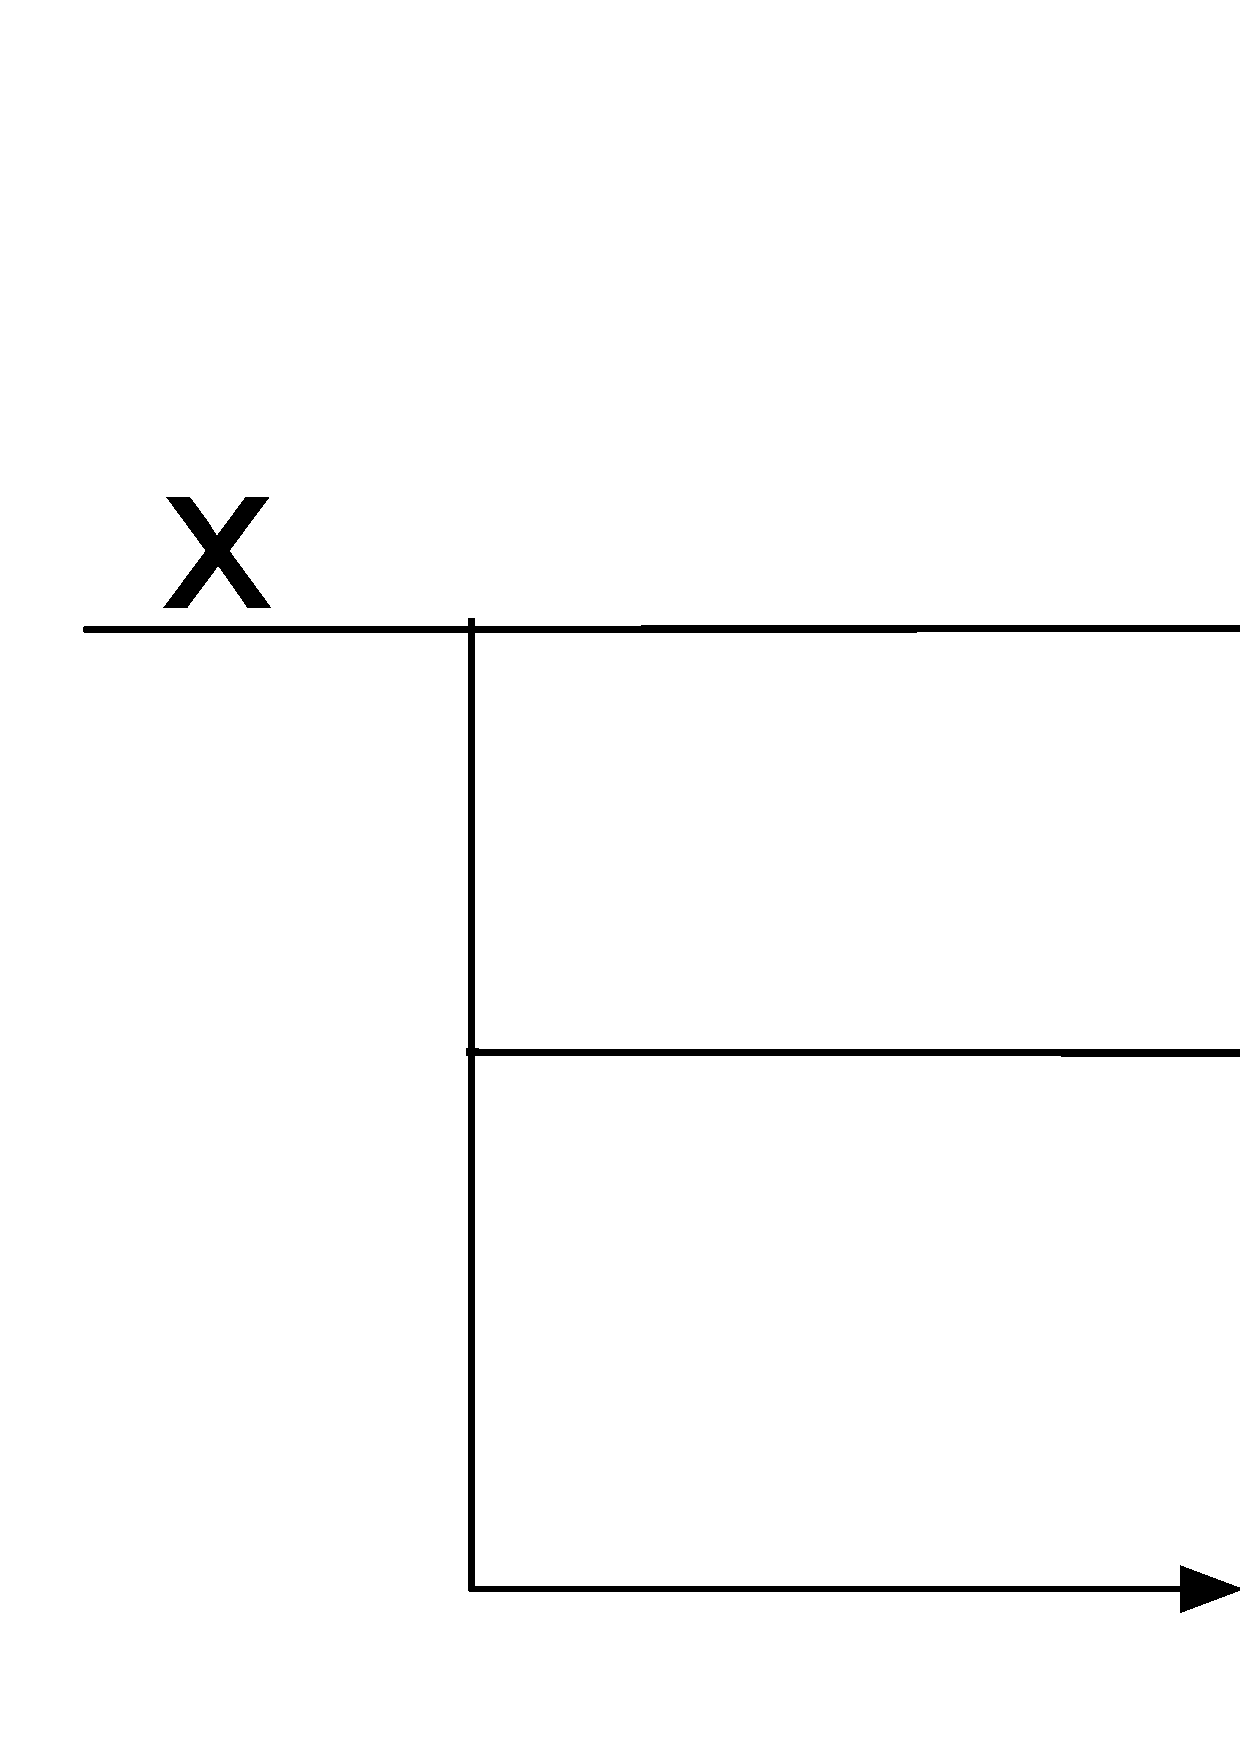
\includegraphics[width=9cm]{TurboEncoder.pdf}
	\end{center}
	
	\begin{itemize}
	\setlength\itemsep{2em}
	\item ターボ符号器の出力の長さ: $(n+1)N$、$R$=$\frac{1}{n+1}$
	
	\item ターボ復号器の出力の長さ: $N$
	
	\end{itemize}


\end{frame}


%Slide 4
\begin{frame}
\frametitle{5. RSC符号と$a\tau$-2エラーイベント}
\begin{figure}
		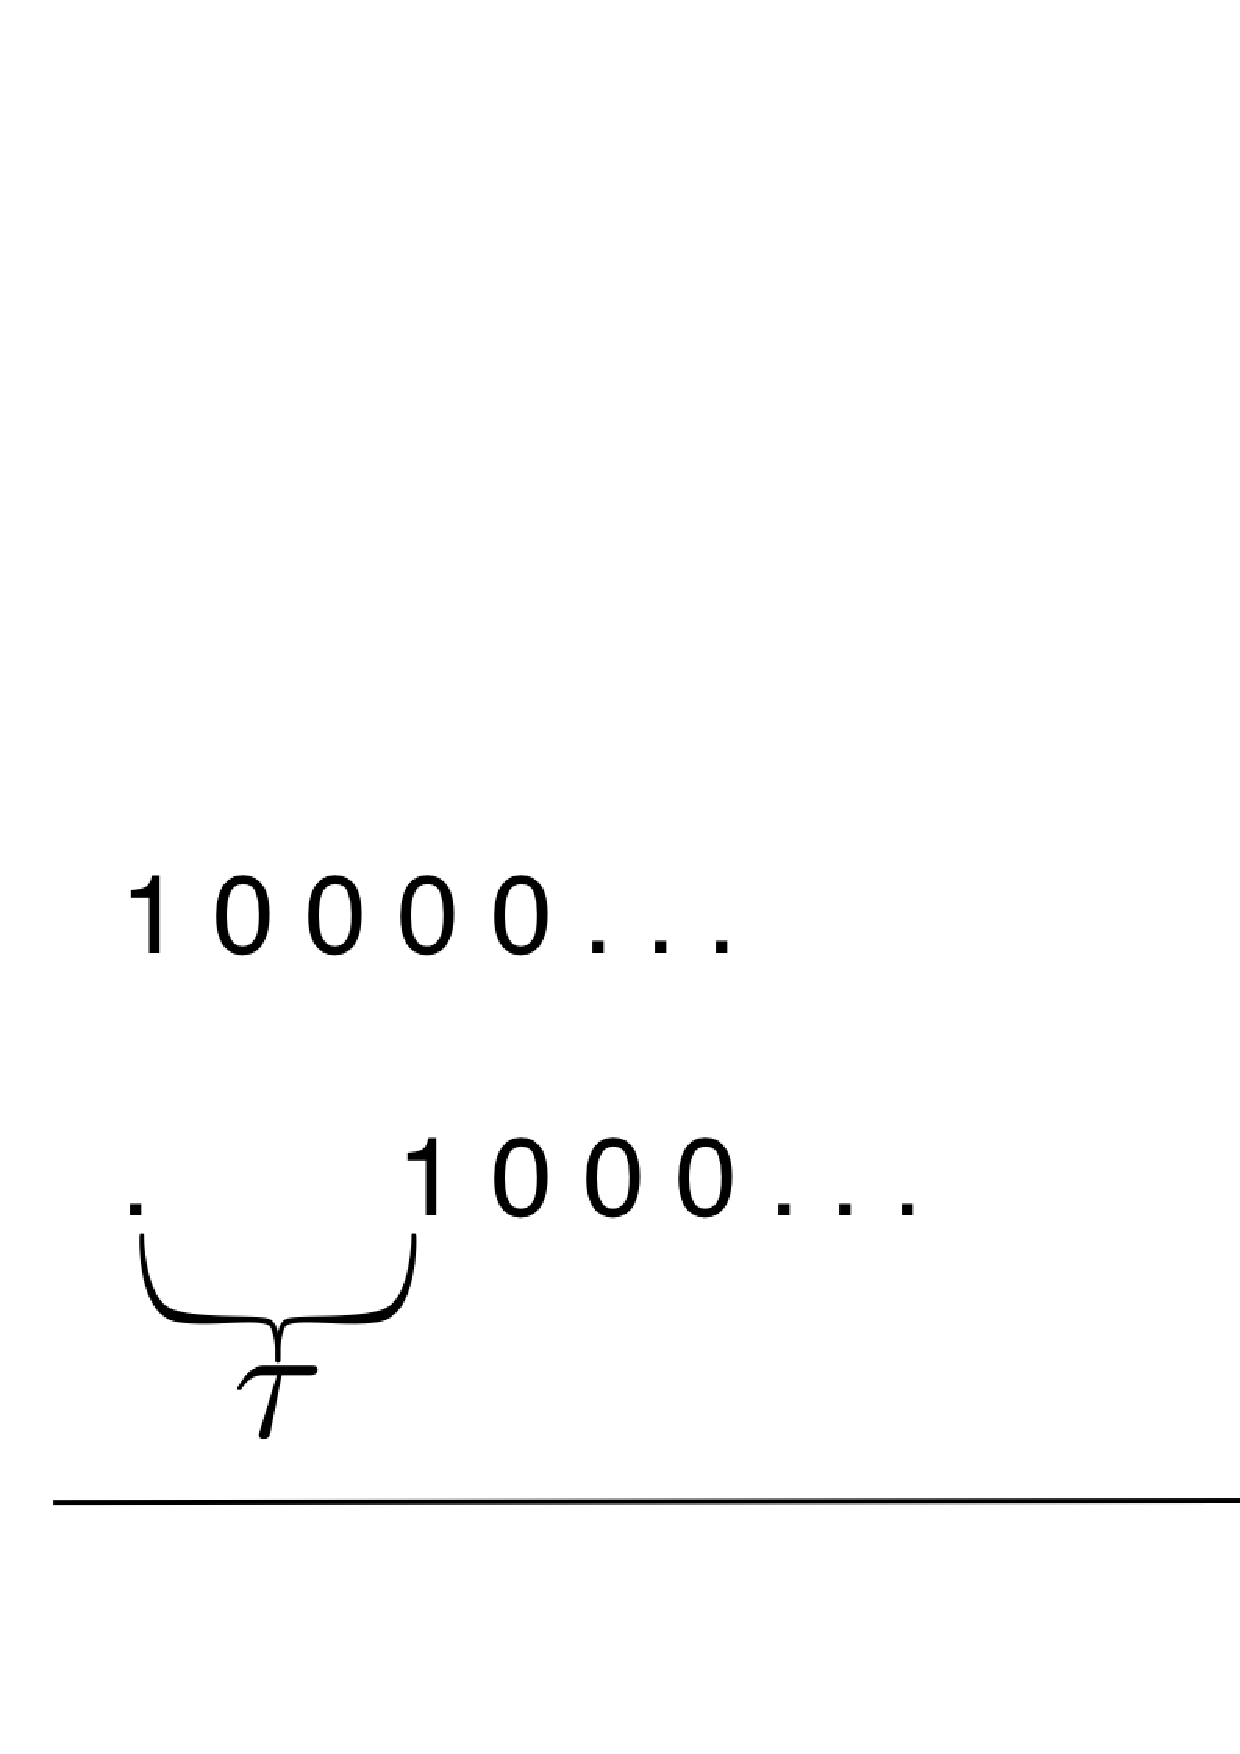
\includegraphics[width=10cm]{RSCExample.pdf}
		\caption{例: 5/7 RSC符号器}
	\end{figure}
\begin{itemize}
\setlength\itemsep{2em}

\item $a\tau$-2エラーイベント: $a\tau$で離れたビット''1''2つを持つ情報系列


$$(1+D^{a\tau})(D^u) \triangleq \mathbb{F}$$
$$0\leq u\leq N-a\tau, a=\{1,2,3,...\}$$


\end{itemize}

\end{frame}
%Slide 5

\begin{frame}
\frametitle{6.  ターボ符号での$a\tau$-2エラーイベント}

\begin{center}
\includegraphics[width=2.5cm]{InterleaverWorking.pdf}
\end{center}

\begin{center}
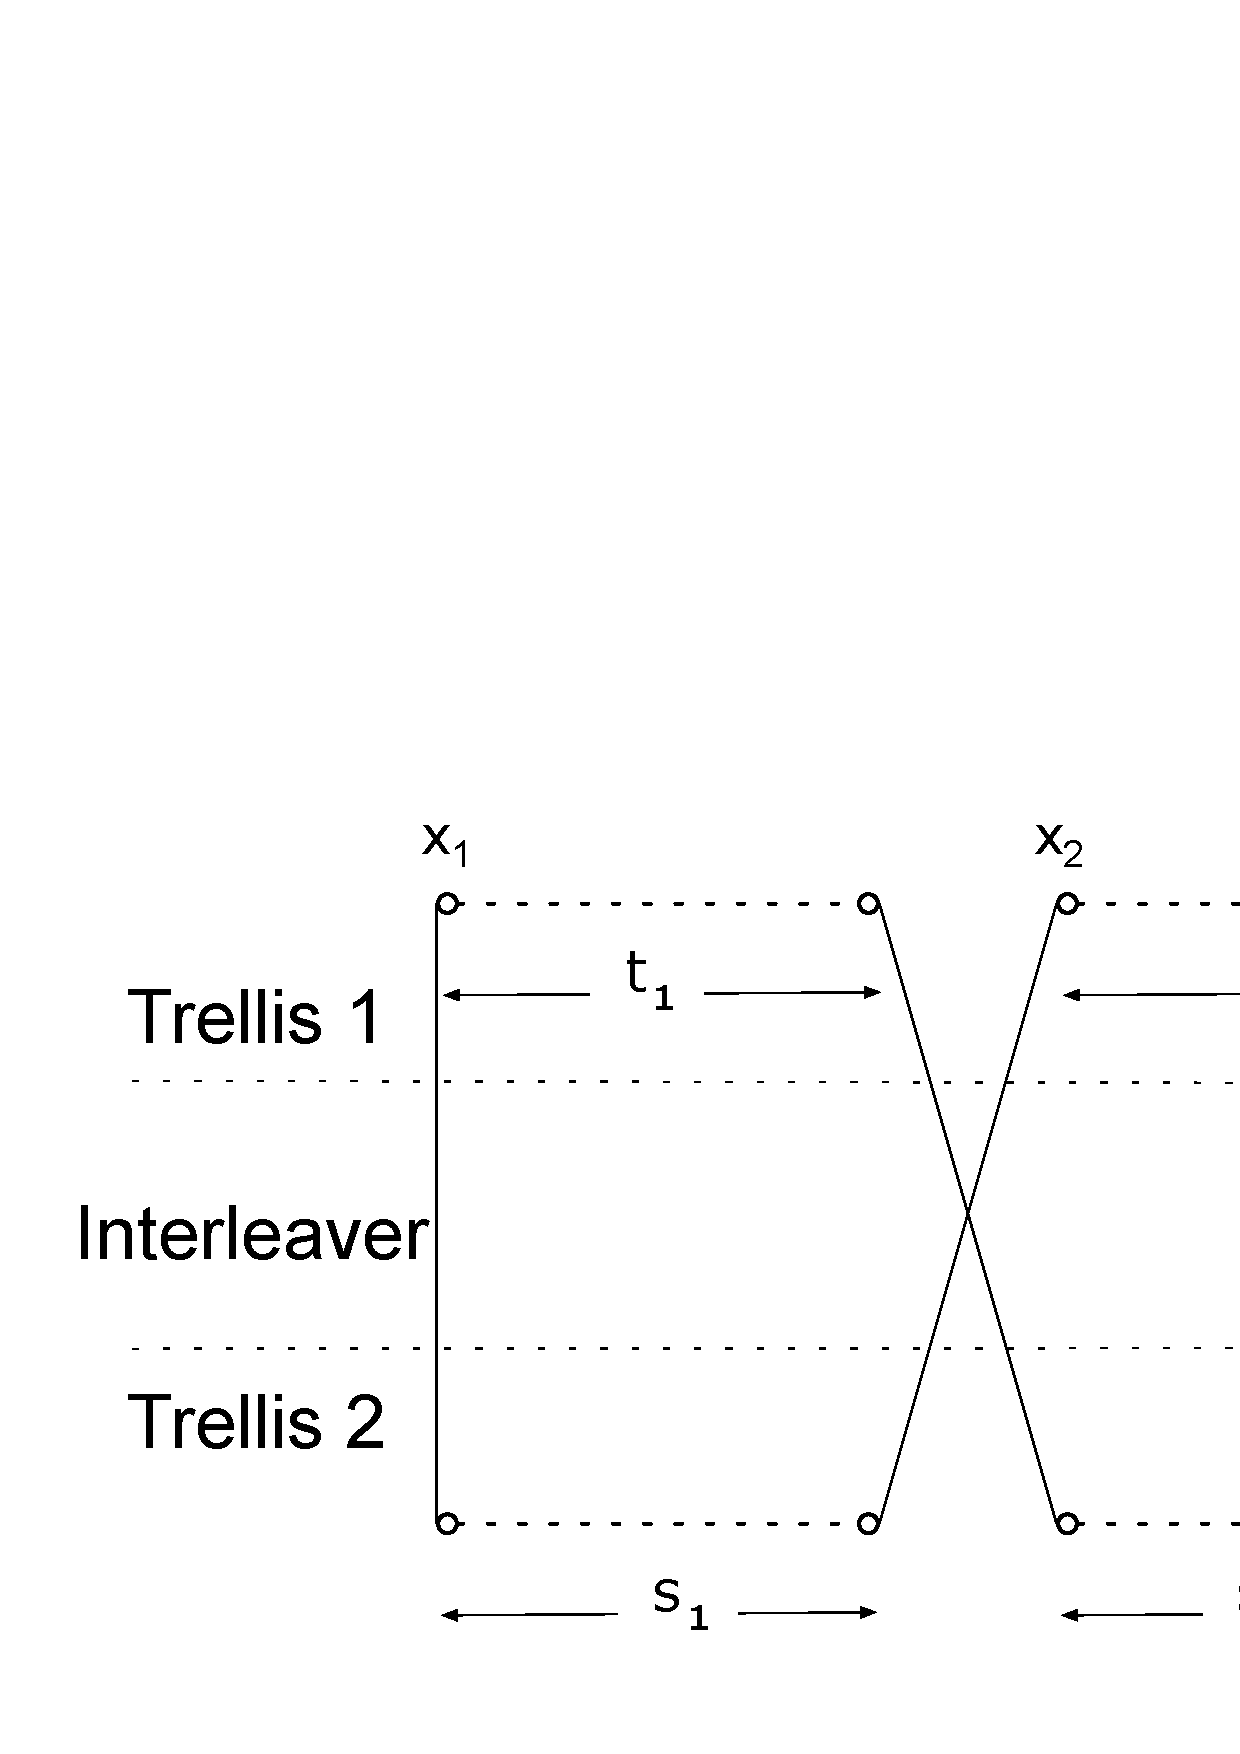
\includegraphics[width=8cm]{weight2m.pdf}
\end{center}

\begin{itemize}
\item  ターボ符号でのエラーイベント: $(t_i,s_j)_v$,RSC符号1:$t_i$, RSC符号2:$s_j$
\end{itemize}


\end{frame}
%Slide 6


\begin{frame}
\frametitle{7. ターボ符号の性能解析}
\setlength\itemsep{2em}

\begin{itemize}
\setlength\itemsep{1em}

\item 符号語の重み

 $$d_{(t_i,s_j)_v}=6m+\Bigg( \frac{ \sum \left|t_i\right|}{\tau} + \frac{ \sum \left|s_j\right|}{\tau} \Bigg)w_o$$

 注意:$(t_i,s_j)_v \in \mathbb{F}$ 

\item ビット誤り率性能の近似式

 $$P_b \approx \sum_{v=1}^{l} \frac{2mN_{d{(t_i,s_j)_v}}}{N}Q\Bigg( \sqrt{d_{(t_i,s_j)_v}\frac{2RE_b}{N_o}}\Bigg)$$



\end{itemize}

\end{frame}
%%%%%%%%%%%%%%%%%%%%%%%%%%%%%%%


\begin{frame}
\frametitle{8. 線形インタリーバの最適化}

\begin{center}
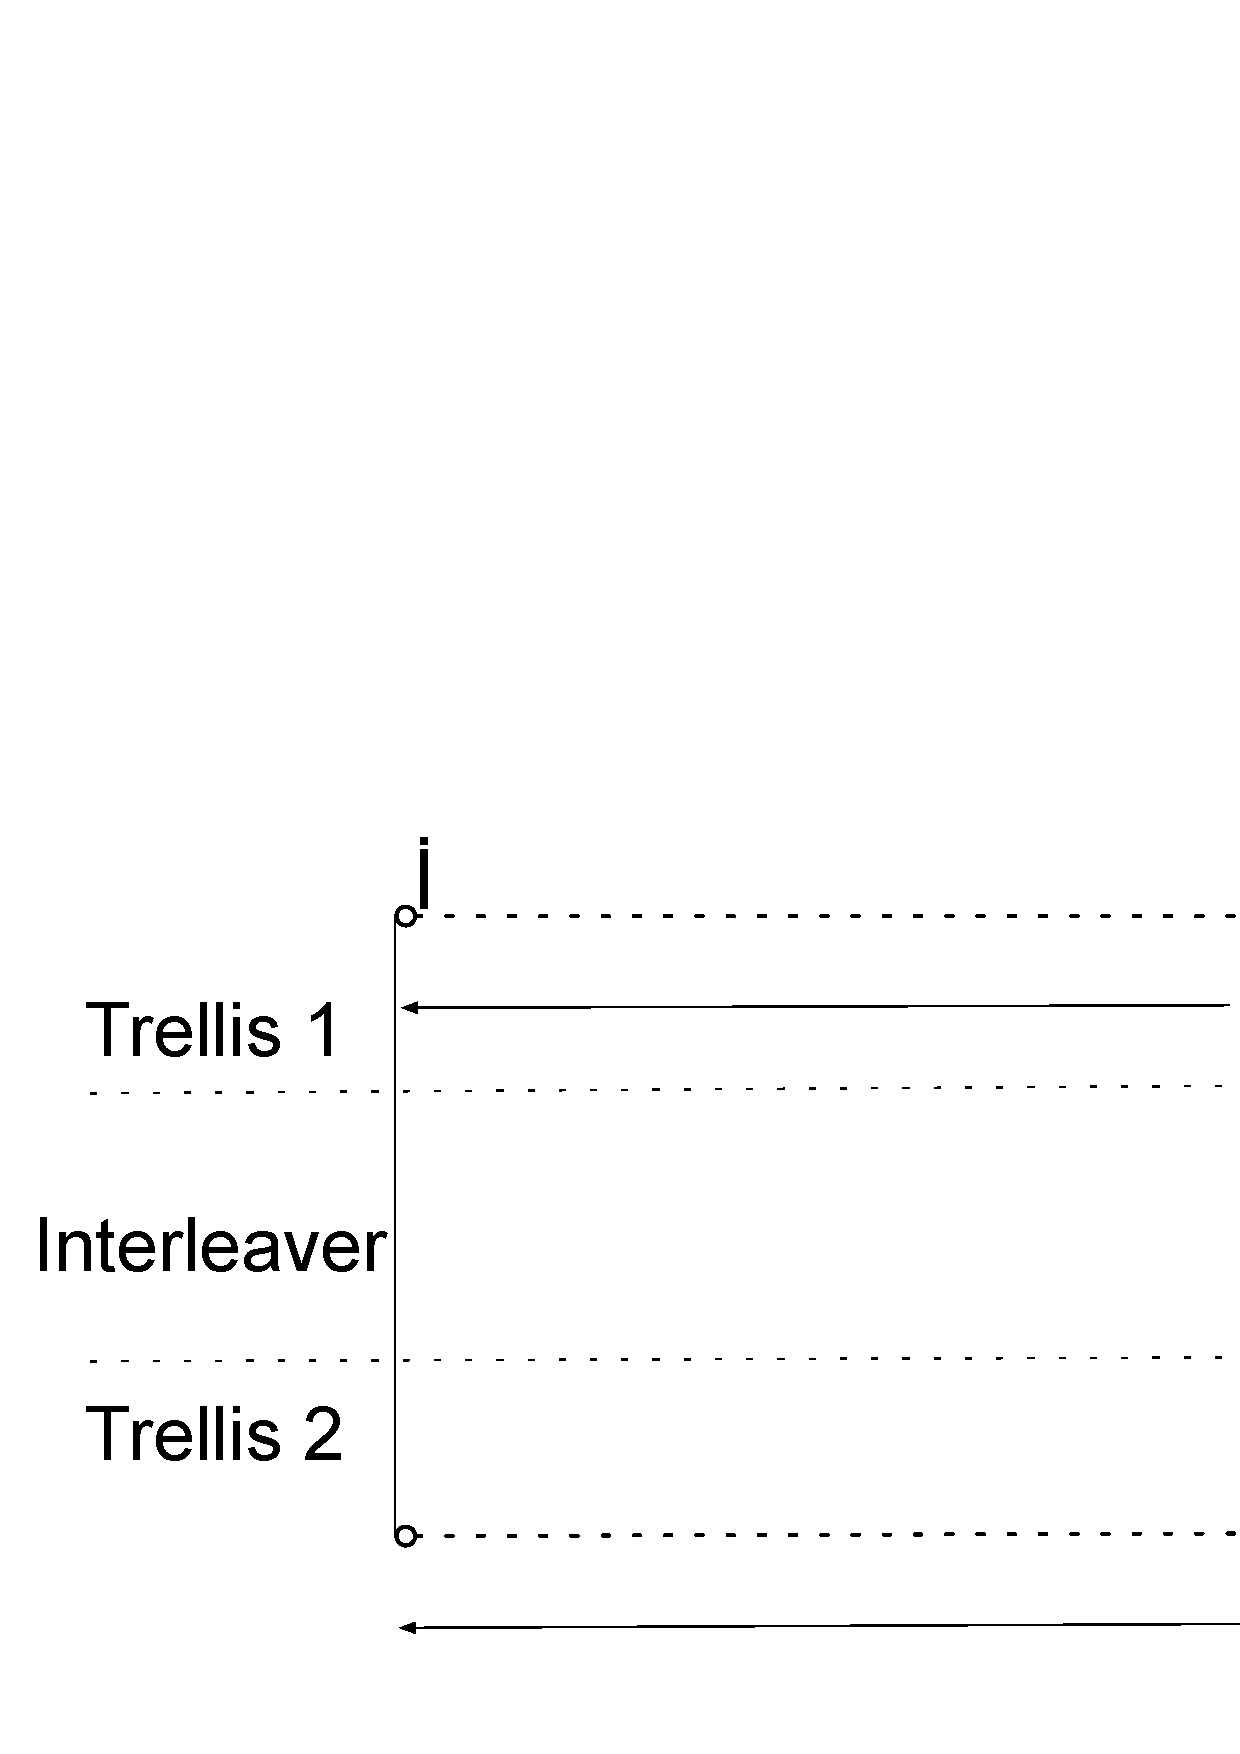
\includegraphics[width=10cm]{weight2.pdf}
\end{center}

\begin{itemize}
\setlength\itemsep{2em}
%\item $d_{ef}$: 2エラーイベントの入力による、符号語の最低距離
\item  $m=1$, $t=s=\tau$の場合を防止したい

\item 線形インタリーバのマッピング関数 
 $$
\Pi_{\mathbf{L}_n}(i) \equiv bi  \mod N, \ 0 \leq i \leq N
$$
\end{itemize}

\end{frame}

%%%
\begin{frame}
\frametitle{9. 最良のbの選択方法}

\begin{itemize}
\setlength\itemsep{2em}
\item bのすべての可能な値で、$\Pi_{\mathbf{L}_n}(i+t)-\Pi_{\mathbf{L}_n}(i)=s$
を計算する

\item $d_{(t_i,s_j)_v}$を計算してmin $d_{(t_i,s_j)_v}$を選ぶ
\item bに関するmax(min $d_{(t_i,s_j)_v}$)を選択する
\begin{itemize}
\setlength\itemsep{1em}
\item 結論:最良のb =>$\tau$と互いに素
\end{itemize}

\end{itemize}

\end{frame}
%%%%
\begin{frame}
\frametitle{10. 進捗状況}
\begin{itemize}
\setlength \itemsep{2em}
\item システムモデルの作成
\item 結論の確認中
\end{itemize}


\end{frame}


\begin{frame}
\frametitle{11. 今後の予定}
\begin{itemize}
\setlength\itemsep{2em}
\item $m=1$で、$t_i=\tau \mapsto s_j=\tau$以外の場合のインタリーバを設計する。 

\item $m=2$で、$t_i=a\tau \mapsto s_j=a\tau $のほかの場合のインタリーバを設計する。
\end{itemize}


\end{frame}



\end{document}
